% This file was converted to LaTeX by Writer2LaTeX ver. 1.0.2
% see http://writer2latex.sourceforge.net for more info
\documentclass[11pt]{article}
\usepackage[utf8]{inputenc}
\usepackage[T1]{fontenc}
\usepackage[english]{babel}
\usepackage{amsmath}
\usepackage{amssymb,amsfonts,textcomp}
\usepackage{array}
\usepackage{supertabular}
\usepackage{hhline}
\usepackage{hyperref}
\hypersetup{colorlinks=true, linkcolor=blue, citecolor=blue, filecolor=blue, urlcolor=blue}
\usepackage{graphicx}
\newcommand\textsubscript[1]{\ensuremath{{}_{\text{#1}}}}
% Text styles
\newcommand\textstyleListLabeli[1]{{\fontsize{12pt}{14.4pt}\selectfont \textrm{\textbf{#1}}}}
\newcommand\textstyleListLabelii[1]{{\fontsize{12pt}{14.4pt}\selectfont \textrm{\textmd{#1}}}}
\newcommand\textstyleFootnoteanchor[1]{\textsuperscript{#1}}
\makeatletter
\newcommand\arraybslash{\let\\\@arraycr}
\makeatother
\raggedbottom
% Paragraph styles
\renewcommand\familydefault{\rmdefault}
\newenvironment{styleStandard}{\setlength\leftskip{0cm}\setlength\rightskip{0cm plus 1fil}\setlength\parindent{0cm}\setlength\parfillskip{0pt plus 1fil}\setlength\parskip{0in plus 1pt}\writerlistparindent\writerlistleftskip\leavevmode\normalfont\normalsize\writerlistlabel\ignorespaces}{\unskip\vspace{0.139in plus 0.0139in}\par}
\newenvironment{styleListParagraph}{\setlength\leftskip{0.5in}\setlength\rightskip{0in plus 1fil}\setlength\parindent{0in}\setlength\parfillskip{0pt plus 1fil}\setlength\parskip{0in plus 1pt}\writerlistparindent\writerlistleftskip\leavevmode\normalfont\normalsize\writerlistlabel\ignorespaces}{\unskip\vspace{0.139in plus 0.0139in}\par}
\newenvironment{styleHSMHeadingA}{\renewcommand\baselinestretch{1.6666666}\setlength\leftskip{0.3937in}\setlength\rightskip{0in}\setlength\parindent{-0.3937in}\setlength\parfillskip{0pt plus 1fil}\setlength\parskip{0in plus 1pt}\writerlistparindent\writerlistleftskip\leavevmode\normalfont\normalsize\fontsize{12pt}{14.4pt}\selectfont\bfseries\writerlistlabel\ignorespaces}{\unskip\vspace{0in plus 1pt}\par}
\newenvironment{styleHSMBlankLine}{\renewcommand\baselinestretch{1.6666666}\setlength\leftskip{0in}\setlength\rightskip{0in}\setlength\parindent{0in}\setlength\parfillskip{0pt plus 1fil}\setlength\parskip{0in plus 1pt}\writerlistparindent\writerlistleftskip\leavevmode\normalfont\normalsize\fontsize{12pt}{14.4pt}\selectfont\writerlistlabel\ignorespaces}{\unskip\vspace{0in plus 1pt}\par}
% List styles
\newcommand\writerlistleftskip{}
\newcommand\writerlistparindent{}
\newcommand\writerlistlabel{}
\newcommand\writerlistremovelabel{\aftergroup\let\aftergroup\writerlistparindent\aftergroup\relax\aftergroup\let\aftergroup\writerlistlabel\aftergroup\relax}
\newcounter{listWWNumileveli}
\newcounter{listWWNumilevelii}[listWWNumileveli]
\newcounter{listWWNumileveliii}[listWWNumilevelii]
\newcounter{listWWNumileveliv}[listWWNumileveliii]
\renewcommand\thelistWWNumileveli{\arabic{listWWNumileveli}}
\renewcommand\thelistWWNumilevelii{\arabic{listWWNumileveli}.\arabic{listWWNumilevelii}}
\renewcommand\thelistWWNumileveliii{\arabic{listWWNumileveli}.\arabic{listWWNumilevelii}.\arabic{listWWNumileveliii}}
\renewcommand\thelistWWNumileveliv{\arabic{listWWNumileveli}.\arabic{listWWNumilevelii}.\arabic{listWWNumileveliii}.\arabic{listWWNumileveliv}}
\newcommand\labellistWWNumileveli{\textstyleListLabeli{\thelistWWNumileveli.}}
\newcommand\labellistWWNumilevelii{\thelistWWNumilevelii.}
\newcommand\labellistWWNumileveliii{\thelistWWNumileveliii.}
\newcommand\labellistWWNumileveliv{\thelistWWNumileveliv.}
\newenvironment{listWWNumileveli}{\def\writerlistleftskip{\addtolength\leftskip{0.0cm}}\def\writerlistparindent{}\def\writerlistlabel{}\def\item{\def\writerlistparindent{\setlength\parindent{-0cm}}\def\writerlistlabel{\stepcounter{listWWNumileveli}\makebox[0cm][l]{\labellistWWNumileveli}\hspace{0cm}\writerlistremovelabel}}}{}
\newenvironment{listWWNumilevelii}{\def\writerlistleftskip{\addtolength\leftskip{0.0cm}}\def\writerlistparindent{}\def\writerlistlabel{}\def\item{\def\writerlistparindent{\setlength\parindent{-0cm}}\def\writerlistlabel{\stepcounter{listWWNumilevelii}\makebox[0cm][l]{\labellistWWNumilevelii}\hspace{0cm}\writerlistremovelabel}}}{}
\newenvironment{listWWNumileveliii}{\def\writerlistleftskip{\addtolength\leftskip{0.0cm}}\def\writerlistparindent{}\def\writerlistlabel{}\def\item{\def\writerlistparindent{\setlength\parindent{-0cm}}\def\writerlistlabel{\stepcounter{listWWNumileveliii}\makebox[0cm][l]{\labellistWWNumileveliii}\hspace{0cm}\writerlistremovelabel}}}{}
\newenvironment{listWWNumileveliv}{\def\writerlistleftskip{\addtolength\leftskip{0.0cm}}\def\writerlistparindent{}\def\writerlistlabel{}\def\item{\def\writerlistparindent{\setlength\parindent{-0cm}}\def\writerlistlabel{\stepcounter{listWWNumileveliv}\makebox[0cm][l]{\labellistWWNumileveliv}\hspace{0cm}\writerlistremovelabel}}}{}
\newcounter{listWWNumvleveli}
\newcounter{listWWNumvlevelii}[listWWNumvleveli]
\newcounter{listWWNumvleveliii}[listWWNumvlevelii]
\newcounter{listWWNumvleveliv}[listWWNumvleveliii]
\renewcommand\thelistWWNumvleveli{\arabic{listWWNumvleveli}}
\renewcommand\thelistWWNumvlevelii{\alph{listWWNumvlevelii}}
\renewcommand\thelistWWNumvleveliii{\roman{listWWNumvleveliii}}
\renewcommand\thelistWWNumvleveliv{\arabic{listWWNumvleveliv}}
\newcommand\labellistWWNumvleveli{\textstyleListLabelii{(\thelistWWNumvleveli)}}
\newcommand\labellistWWNumvlevelii{\thelistWWNumvlevelii.}
\newcommand\labellistWWNumvleveliii{\thelistWWNumvleveliii.}
\newcommand\labellistWWNumvleveliv{\thelistWWNumvleveliv.}
\newenvironment{listWWNumvleveli}{\def\writerlistleftskip{\addtolength\leftskip{0.0cm}}\def\writerlistparindent{}\def\writerlistlabel{}\def\item{\def\writerlistparindent{\setlength\parindent{-0cm}}\def\writerlistlabel{\stepcounter{listWWNumvleveli}\makebox[0cm][l]{\labellistWWNumvleveli}\hspace{0cm}\writerlistremovelabel}}}{}
\newenvironment{listWWNumvlevelii}{\def\writerlistleftskip{\addtolength\leftskip{0.0cm}}\def\writerlistparindent{}\def\writerlistlabel{}\def\item{\def\writerlistparindent{\setlength\parindent{-0cm}}\def\writerlistlabel{\stepcounter{listWWNumvlevelii}\makebox[0cm][l]{\labellistWWNumvlevelii}\hspace{0cm}\writerlistremovelabel}}}{}
\newenvironment{listWWNumvleveliii}{\def\writerlistleftskip{\addtolength\leftskip{0.0cm}}\def\writerlistparindent{}\def\writerlistlabel{}\def\item{\def\writerlistparindent{\setlength\parindent{-0cm}}\def\writerlistlabel{\stepcounter{listWWNumvleveliii}\makebox[0cm][r]{\labellistWWNumvleveliii}\hspace{0cm}\writerlistremovelabel}}}{}
\newenvironment{listWWNumvleveliv}{\def\writerlistleftskip{\addtolength\leftskip{0.0cm}}\def\writerlistparindent{}\def\writerlistlabel{}\def\item{\def\writerlistparindent{\setlength\parindent{-0cm}}\def\writerlistlabel{\stepcounter{listWWNumvleveliv}\makebox[0cm][l]{\labellistWWNumvleveliv}\hspace{0cm}\writerlistremovelabel}}}{}
\setlength\tabcolsep{1mm}
\renewcommand\arraystretch{1.3}
% footnotes configuration
\makeatletter
\renewcommand\thefootnote{\arabic{footnote}}
\renewcommand\@makefnmark{\mbox{\textstyleFootnoteanchor{\@thefnmark}}}
\makeatother
\title{}
\author{Maria del Mar Vanrell Bosch}
\date{2015-11-28}
\begin{document}
\clearpage\setcounter{page}{1}\begin{styleStandard}
\textbf{Language variation at the prosody-syntax interface: Focus in European Spanish}
\end{styleStandard}


\begin{styleStandard}
Maria del Mar Vanrell and Olga Fernández-Soriano 
\end{styleStandard}


\begin{styleStandard}
Freie Universität Berlin and Universidad Autónoma de Madrid
\end{styleStandard}


\begin{styleStandard}
mariadelmar.vanrell@fu-berlin.de and olga.fernandez@uam.es
\end{styleStandard}


\begin{styleStandard}
\textbf{Abstract}
\end{styleStandard}


\begin{styleStandard}
Spanish is generally considered a “Word Order Language” in the marking of focus. The syntactic strategies used to change the canonical word order seem to depend on focus type. Thus, prosodically motivated movement is proposed for information narrow focus, and focus fronting, clefting or focus in situ for contrastive focus. However, recent empirical studies do not fully agree with this assumption. This article investigates the effect of language variation and other factors such as focus type and focused constituent on the syntactic and phonological realization of focus in European Spanish. Our data demonstrate that Spanish resorts to both word order and intonation to different degrees depending especially on the language variety, but also on the focused constituent (subject or object) and the focus type (information and contrastive narrow focus). 
\end{styleStandard}


\begin{styleStandard}
\textit{Key words: }language variation, focus, syntax, phonology, European Spanish
\end{styleStandard}


\setcounter{listWWNumileveli}{0}
\begin{listWWNumileveli}
\item 
\begin{styleListParagraph}
\textbf{Introduction}
\end{styleListParagraph}

\end{listWWNumileveli}
\begin{styleListParagraph}
It is generally assumed that Spanish as well as other Romance languages like Italian resorts to syntactic movement to mark focus (Bolinger 1954, 1954-55, Contreras 1978, 1980, Büring \& Gutiérrez-Bravo 2001, Büring 2010, Domínguez 2004a, 2004b, Gutiérrez-Bravo 2002, 2008, Ordóñez 2000, Zubizarreta 1998). The specific strategies used to alter the canonical word order seem to depend on the focus type. Thus, according to Contreras (1976) or Zubizarreta (1998, 1999) information focus has to be in sentence-final- position, where it receives the main prominence of the sentence or nuclear accent by means of the Nuclear Stress Rule (NSR) (Chomsky and Halle 1968, Zubizarreta 1998). Given that \textit{prominence/stress shift} (also called focus prosodically marked in situ) seems not to be an available strategy in Spanish (see (1b)), in this language the non-focal material has to move to a non-canonical position (\textit{prosodically motivated movement} or \textit{p-movement}) (see (1c)) to ensure that the element the speaker wishes to focalize appears in the rightmost position.
\end{styleListParagraph}


\setcounter{listWWNumvleveli}{0}
\begin{listWWNumvleveli}
\item 
\begin{styleListParagraph}
a.\textit{¿Qué trajo Blancanieves?}
\end{styleListParagraph}

\end{listWWNumvleveli}
\begin{styleListParagraph}
what bring.\textsc{past.3sg} Snow.White
\end{styleListParagraph}


\begin{styleListParagraph}
‘What did Snow White bring?’
\end{styleListParagraph}


\begin{styleListParagraph}
b. \textit{*[Blancanieves]}\textit{\textsubscript{F}}\textit{ trajo manzanas}
\end{styleListParagraph}


\begin{styleListParagraph}
Snow.White bring.\textsc{past.3sg} apples
\end{styleListParagraph}


\begin{styleListParagraph}
‘Snow White brought apples’
\end{styleListParagraph}


\begin{styleListParagraph}
c. \textit{Trajo manzanas [Blancanieves]}\textit{\textsubscript{F}}
\end{styleListParagraph}


\begin{styleListParagraph}
bring.\textsc{past.3sg} apples Snow.White
\end{styleListParagraph}


\begin{styleListParagraph}
‘Snow White brought apples’
\end{styleListParagraph}


\begin{styleHSMHeadingA}
\textmd{Whereas in Spanish information focus declaratives just p-movement is applied as an alternative strategy to prominence shift, according to Zubizarreta (1998, 1999) a variety of mechanisms are available for contrastive focus (see (2)). Thus, the focused constituent can be clefted (as in (2b)), fronted (as in (2c)) or remain in situ (see (2d)). It is most commonly claimed that in all the sentences in (2b-d) the focused constituent, }\textmd{\textit{manzanas}}\textmd{ ‘apples’, bears the nuclear accent.}
\end{styleHSMHeadingA}


\begin{listWWNumvleveli}
\item 
\begin{styleHSMHeadingA}
\textmd{a. }\textmd{\textit{Blancanieves trajo pomelos, ¿no?}}
\end{styleHSMHeadingA}

\end{listWWNumvleveli}
\begin{styleHSMHeadingA}
\textmd{Snow.White bring.}\textmd{\textsc{past.3sg}}\textmd{ grapefruits no}
\end{styleHSMHeadingA}


\begin{styleHSMHeadingA}
\textmd{‘Snow White brought grapefruits, right?’}
\end{styleHSMHeadingA}


\begin{styleHSMHeadingA}
\textmd{b}\textmd{\textit{. No, fue [manzanas]}}\textit{\textsubscript{CF}}\textmd{\textit{ lo que trajo Blancanieves}}
\end{styleHSMHeadingA}


\begin{styleHSMHeadingA}
\textmd{no was apples }\textmd{\textsc{art}}\textmd{ that bring.}\textmd{\textsc{past.3sg}}\textmd{ Snow.White}
\end{styleHSMHeadingA}


\begin{styleHSMHeadingA}
\textmd{‘No, it was }\textmd{apples}\textmd{ that Snow White brought’}
\end{styleHSMHeadingA}


\begin{styleHSMHeadingA}
\textmd{c. }\textmd{\textit{No, [manzanas]}}\textit{\textsubscript{CF}}\textmd{\textit{ trajo Blancanieves}}
\end{styleHSMHeadingA}


\begin{styleHSMHeadingA}
\textmd{no apples bring.}\textmd{\textsc{past.3sg }}\textmd{Snow.White}
\end{styleHSMHeadingA}


\begin{styleHSMHeadingA}
\textmd{‘No, Snow White brought }\textmd{apples}\textmd{’}
\end{styleHSMHeadingA}


\begin{styleHSMHeadingA}
\textmd{d. }\textmd{\textit{No, Blancanieves trajo [manzanas]}}\textit{\textsubscript{CF}}
\end{styleHSMHeadingA}


\begin{styleHSMHeadingA}
\textmd{no Snow.White bring.}\textmd{\textsc{past.3sg }}\textmd{apples}
\end{styleHSMHeadingA}


\begin{styleHSMHeadingA}
\textmd{‘No, Snow White brought }\textmd{apple}\textmd{s’}
\end{styleHSMHeadingA}


\begin{styleListParagraph}
\ \ This functional division of labor between different syntactic strategies and focus types might not be as clear-cut as proposed in the previous literature. First, recent empirical studies (Gabriel et al. 2009, Gabriel 2010 for Argentinean Spanish; Muntendam 2009, 2013 for Andean Spanish; Leal-Méndez \& Shea 2012 and Hoot 2012a,b for Mexican Spanish; Vanrell \& Fernández-Soriano 2013 for Basque and Canarian Spanish; Jiménez-Fernández submitted for Southern Peninsular Spanish) demonstrate: (a) information focus constituents in Spanish can also remain in situ even if they are not VP-internal (Gabriel et al. 2009, Gabriel 2010, Muntendam 2009, 2013, Leal-Méndez \& Shea 2012, Hoot 2012a,b and Vanrell \& Fernández-Soriano 2013), and (b) focus fronting is not restricted to contrast (Jiménez-Fernández submitted and Vanrell \& Fernández-Soriano 2013). Second, although according to Zubizarreta (1999: 4242), clefting is reserved for those cases implying the rejection of an alternative (contrastive/corrective focus), Moreno Cabrera (1999)\footnote{ Moreno Cabrera (1999) distinguishes three types of clefts: PdR COP-CES or relative clauses which present the copula in the first position (also called \textit{it-clefts}), PdR RL- or clauses with the relative clause in initial-sentence position (\textit{pseudo-clefts}) and PdR CES- or sentences with the clefted clause in the first position (\textit{inverted pseudo-clefts}). Interestingly, according to this author, different types of cleft structures correspond to different information structures. Thus, \textit{it-clefts} tend to be used in contrastive contexts (\textit{contextos posespecificativos} according to his terminology), whereas pseudo-clefts and inverted pseudo-clefts are common in neutral contexts (or \textit{contextos especificativos}).\par \par \par }, Dufter (2009) and Feldhausen \& Vanrell (forthcoming) demonstrate that different types of clefted constructions (it-clefts, pseudo-clefts and inverted pseudo-clefts) can be related to different focal structures.
\end{styleListParagraph}


\begin{styleListParagraph}
\ \ In the prosodic literature on focus marking in Spanish, no special emphasis has been placed upon the different syntactic strategies and how these interact with prosody, but upon the pitch accent choice of the focus stretch or upon how the focal material is marked off from the non-focal material. No intonational difference between information and contrastive focus has been reported (Estebas-Vilaplana \& Prieto 2008, Hualde \& Prieto 2015). As far as deaccentuation of the postfocal material is concerned, it is still a matter of debate. Whereas it has been generally assumed that Romance languages do not deaccent postfocal material in the same way as Germanic languages do (Cruttenden 1993, Swerts et al. 2002, Ladd 2008, among others), acoustic analysis of the postfocal stretch in Spanish reveals suprasegmental hypoarticulation (lower intensity and F0 range), suggesting that deaccentuation does exist in this language (Nadeu \& Vanrell 2015). Since this topic is out of the scope of this paper, we will just use postfocal compression/reduction in a general sense.
\end{styleListParagraph}


\begin{styleStandard}
\ \ Still from a prosodic perspective, it is often claimed that the main correlate of focus is prominence and that alignment is a consequence of it (Büring 2010, Truckenbrodt 1995, Zubizarreta 1998, among others). In this paper we will test, with our experimental data, the conception put forward by Féry (2013). According to this author, alignment and prominence are two different prosodic mechanisms to mark focus, which can cooperate, but do not need to. She also predicts that foci that are “stronger” in the hierarchy (i.e., contrastive/corrective foci), have a stronger tendency to be accompanied by additional phonetic correlates (Féry 2013: 729). Féry illustrates her theory of prosodic focus realization through different languages arguing that different languages may achieve alignment in various ways.
\end{styleStandard}


\begin{styleStandard}
Subject/non-subject asymmetries have been attested in Spanish (Büring \& Gutiérrez-Bravo 2001, Zubizarreta 1998). These are also called subject/object asymmetries, and indicate that subject focus, compared to non-subject focus, always requires a special marking (marking asymmetry) or is realized differently from focused non-subjects (structural asymmetry). According to Fiedler et al. (2010), the reason for this asymmetry is that with this special marking, languages avoid the default interpretation of subjects as topics. Since in our data we controlled for the focused constituent (either subject or direct object), we will be able to test whether these asymmetries are also present in our data.
\end{styleStandard}


\begin{styleStandard}
Traditional studies of Spanish dialectology tend to focus on lexicon and phonology. However, very few studies have looked at the syntax-prosody interface. Coming back to the inconsistencies found between the predictions made by Zubizarreta (1998, 1999) and the results by Gabriel et al. (2009), Muntendam (2009), Jiménez-Fernández (forthcoming), among others, one could hypothesize that this is due to diatopic variation (since the varieties explored in the studies which cast doubt on the predictions made by Zubizarreta (1998, 1999) are different from Castilian Spanish). However, these inconsistencies might also be related to methodology, since only recent work on focus and the prosody-syntax interface in Spanish relies on experimental data (Zubizarreta’s data were based on speakers’ intuitions). In this context and based on the observations by Uth (2014), we also want to test the accuracy of the methodology used in this paper to answer the research questions.
\end{styleStandard}


\begin{styleStandard}
In this paper, the following research questions will be addressed:
\end{styleStandard}


\begin{styleStandard}
RQ1.\ \ Can Spanish still be considered a “Word Order Language” in the marking of focus?
\end{styleStandard}


\begin{styleListParagraph}
RQ2.\ \ Can a clear-cut description be drown of focus types and corresponding different syntactic or phonological strategies? Do these syntactic or phonological mechanisms constitute evidence in favor of the view that alignment and prominence should be treated as two separate phenomena (Féry 2013)?
\end{styleListParagraph}


\begin{styleListParagraph}
RQ3.\ \ Which is the role of language variation in the expression of focus?
\end{styleListParagraph}


\begin{styleStandard}
RQ4.\ \ Can semi-spontaneous picture-based experiments be profitably used to investigate focus at the syntax-prosody interface?
\end{styleStandard}


\begin{styleStandard}
This article is organized as follows. Section 2 describes the methodology used for the production experiment as well as for the prosodic and syntactic annotation of the data. Section 3 presents the main findings of the experiment according to focus type, focused constituent and language variety. Finally, section 4 discusses the main implications of our findings for a better understanding of focal typology in Spanish.
\end{styleStandard}


\setcounter{listWWNumileveli}{0}
\begin{listWWNumileveli}
\item 
\begin{styleListParagraph}
\textbf{Methodology}
\end{styleListParagraph}


\setcounter{listWWNumilevelii}{0}
\begin{listWWNumilevelii}
\item 
\begin{styleListParagraph}
\textbf{Participants}
\end{styleListParagraph}

\end{listWWNumilevelii}
\end{listWWNumileveli}
\begin{styleStandard}
6 women and 2 men aged between 22 and 45 participated in the experiment. They spoke different varieties of European Spanish: 2 female Basque Spanish L1-Basque speakers (from the locales of Gernika and Zeberio, province of Biscay), 2 female Basque Spanish L1-Spanish speakers (from Bilbao, province of Biscay), 2 female Castilian Spanish speakers (from Madrid), 2 male Canarian Spanish speakers (from Las Palmas, province of Las Palmas). The participants were recruited from colleagues of the authors of this paper. They had to be native speakers either of Spanish, or Basque in the specific case of the Basque Spanish speakers-L1 Basque. See Figure 1 for a map including the locales where the recordings were carried out.
\end{styleStandard}


\begin{styleStandard}
  [Warning: Image ignored] % Unhandled or unsupported graphics:
%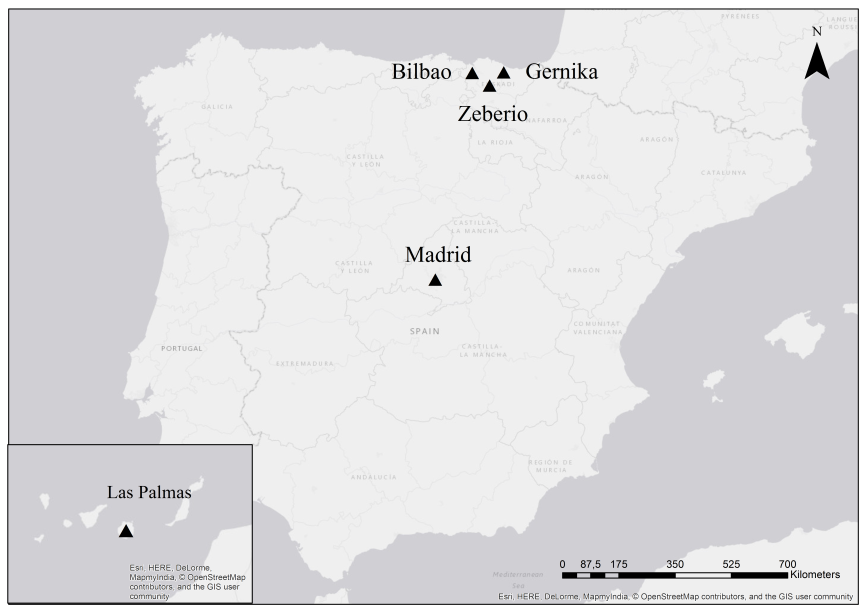
\includegraphics[width=3.9374in,height=2.7866in,width=\textwidth]{VanrellFernandezSorianoFocusEuropeanSpanish-img1.png}
 
\end{styleStandard}


\begin{styleStandard}
Figure 1. Map including the locales where the recordings were carried out. 
\end{styleStandard}


\begin{listWWNumileveli}
\item 
\setcounter{listWWNumilevelii}{0}
\begin{listWWNumilevelii}
\item 
\begin{styleListParagraph}
\textbf{Materials}
\end{styleListParagraph}

\end{listWWNumilevelii}
\end{listWWNumileveli}
\begin{styleListParagraph}
The corpus presented in this paper was elicited through question-answer pairs from short picture stories presented in a PowerPoint slide show (similar to the one used by Gabriel 2010). Different main characters participated in the short stories: a girl called \textit{María}, the fictional character Snow White and a sailor. These short stories corresponded to full sentences with a canonical syntactic structure: subject, verb, direct object and indirect object/adjunct (see (3)).
\end{styleListParagraph}


\setcounter{listWWNumvleveli}{0}
\begin{listWWNumvleveli}
\item 
\begin{styleListParagraph}
\textit{El marinero escribió la carta en el balcón. Después, se la llevó sin permiso.}
\end{styleListParagraph}

\end{listWWNumvleveli}
\begin{styleListParagraph}
the sailor write.\textsc{past.3sg} the letter in the balcony afterwards \textsc{refl} it take.\textsc{past.3sg} without permission
\end{styleListParagraph}


\begin{styleListParagraph}
‘The sailor wrote the letter at the balcony. Afterwards he took it without permission.’
\end{styleListParagraph}


\begin{styleListParagraph}
After the presentation of the pictures (see Figure 2), the participants were asked to respond to a series of wh-questions or tag questions specifically designed to elicit broad and information/contrastive narrow focus on the different constituents (as in (4)). No mirative foci are considered. We take the view that information focus is the answer to a wh- question, whereas contrastive focus “marks a constituent that is a direct rejection of an alternative” (Gussenhoven 2007: 91). Participants were also requested to use all the constituents that appeared in the short stories, but they were totally free to use any syntactic order or strategy as long as they sounded natural. The stories were presented visually, but the first time also in writing. 
\end{styleListParagraph}


\begin{styleListParagraph}
  [Warning: Image ignored] % Unhandled or unsupported graphics:
%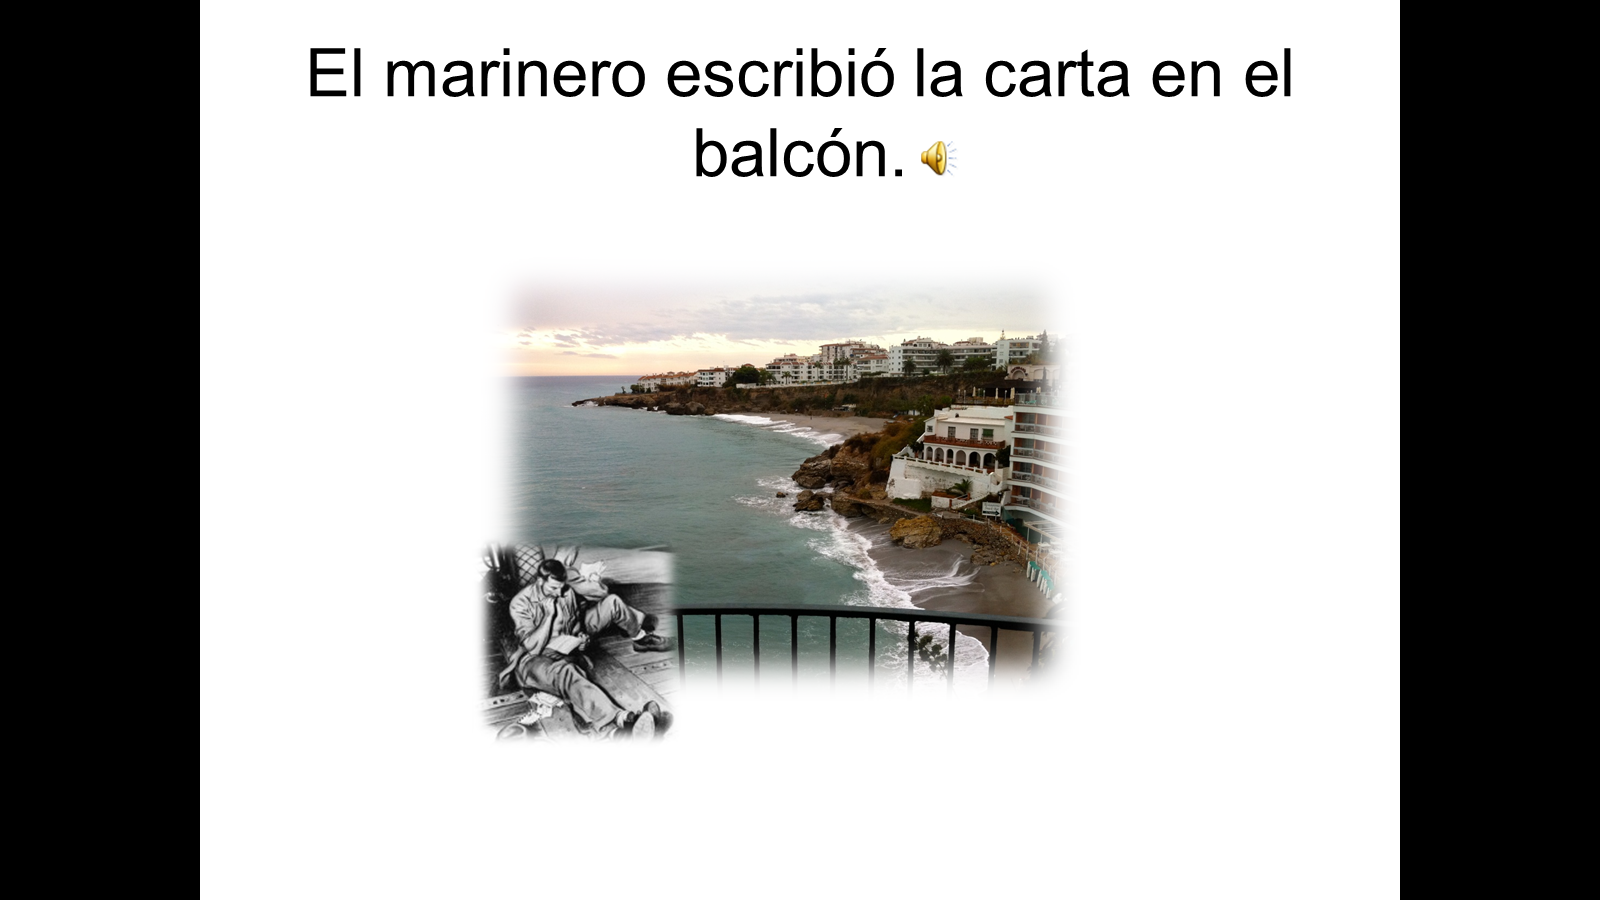
\includegraphics[width=3.05in,height=2.3165in,width=\textwidth]{VanrellFernandezSorianoFocusEuropeanSpanish-img2.png}
 
\end{styleListParagraph}


\begin{styleListParagraph}
Figure 2. Picture of the first part of the story exemplified in (1).
\end{styleListParagraph}


\begin{listWWNumvleveli}
\item 
\begin{styleListParagraph}
a. \textit{¿Qué ha pasado?}
\end{styleListParagraph}

\end{listWWNumvleveli}
\begin{styleListParagraph}
what have.pres.3sg happened
\end{styleListParagraph}


\begin{styleListParagraph}
‘What happened?’
\end{styleListParagraph}


\begin{styleListParagraph}
b. \textit{¿Qué escribió el marinero en el balcón?}
\end{styleListParagraph}


\begin{styleListParagraph}
what write.\textsc{past.3sg} the sailor in the balcony
\end{styleListParagraph}


\begin{styleListParagraph}
‘What did the sailor write on the balcony?’
\end{styleListParagraph}


\begin{styleListParagraph}
c. \textit{¿Quién escribió la carta en el balcón?}
\end{styleListParagraph}


\begin{styleListParagraph}
who write.\textsc{past.3sg} the letter in the balcony
\end{styleListParagraph}


\begin{styleListParagraph}
‘Who wrote the letter on the balcony?’
\end{styleListParagraph}


\begin{styleListParagraph}
d. \textit{El marinero escribió en el balcón la canción, ¿verdad?}
\end{styleListParagraph}


\begin{styleListParagraph}
the sailor write.\textsc{past.3sg }in the balcony the song right
\end{styleListParagraph}


\begin{styleListParagraph}
‘The sailor wrote a song on the balcony, right?’
\end{styleListParagraph}


\begin{styleListParagraph}
e. \textit{¿Dónde escribió la carta el marinero?}
\end{styleListParagraph}


\begin{styleListParagraph}
where write.\textsc{past.3sg }the letter the sailor
\end{styleListParagraph}


\begin{styleListParagraph}
‘Where did the sailor write the letter?’
\end{styleListParagraph}


\begin{styleListParagraph}
f. \textit{Escribió la carta en el balcón el capitán, ¿verdad?}
\end{styleListParagraph}


\begin{styleListParagraph}
write.\textsc{past.3sg }the letter in the balcony the captain right
\end{styleListParagraph}


\begin{styleListParagraph}
‘The captain wrote the letter on the balcony, right?’
\end{styleListParagraph}


\begin{styleListParagraph}
g\textit{.}\textit{¿Qué hizo el marinero con la carta?}
\end{styleListParagraph}


\begin{styleListParagraph}
what do.\textsc{past.3sg} the sailor with the letter
\end{styleListParagraph}


\begin{styleListParagraph}
‘What did the sailor do with the letter?’
\end{styleListParagraph}


\begin{styleListParagraph}
h. \textit{El marinero escribió la carta en la barca, ¿no?}
\end{styleListParagraph}


\begin{styleListParagraph}
the sailor write.\textsc{past.3sg }the letter in the boat no
\end{styleListParagraph}


\begin{styleListParagraph}
‘The sailor wrote the letter on the boat, didn’t he?’
\end{styleListParagraph}


\begin{styleListParagraph}
i. \textit{¿Qué hizo el marinero en el balcón?}
\end{styleListParagraph}


\begin{styleListParagraph}
what do.\textsc{past.3sg} the sailor in the balcony
\end{styleListParagraph}


\begin{styleListParagraph}
‘What did the sailor do on the balcony?’
\end{styleListParagraph}


\begin{styleListParagraph}
j. \textit{El marinero firmó la carta en el balcón, ¿verdad?}
\end{styleListParagraph}


\begin{styleListParagraph}
the sailor sign.\textsc{past.3sg} the letter in the balcony right
\end{styleListParagraph}


\begin{styleListParagraph}
‘The sailor signed the letter on the balcony, right? ’
\end{styleListParagraph}


\begin{styleListParagraph}
k. \textit{La carta, la escribió en el balcón el capitán, ¿no?}
\end{styleListParagraph}


\begin{styleListParagraph}
the letter it write.\textsc{past.3sg} in the balcony the captain no
\end{styleListParagraph}


\begin{styleListParagraph}
‘The captain wrote the letter on the balcony, didn’t he?’
\end{styleListParagraph}


\begin{styleStandard}
The total data obtained through this method was 1056 contours (22 contours x 3 stories x 4 Spanish varieties x 2 speakers).
\end{styleStandard}


\setcounter{listWWNumileveli}{0}
\begin{listWWNumileveli}
\item 
\setcounter{listWWNumilevelii}{0}
\begin{listWWNumilevelii}
\item 
\begin{styleListParagraph}
\textbf{Procedure}
\end{styleListParagraph}

\end{listWWNumilevelii}
\end{listWWNumileveli}
\begin{styleListParagraph}
The researchers set up the recording equipment and were close to the participants at the beginning of the recording session in order to solve potential problems, but then the researchers occupied a peripheral position in the room, so that the participants performed the experiment at their own pace. The experiment lasted approximately 30 minutes. Speakers were recorded on Zoom H4n digital audio recorder using an AKG C520 condenser microphone. All the speakers were recorded in a relaxed atmosphere in their homes with the exception of Canarian speakers, which were recorded at the Universidad de Las Palmas de Gran Canaria.
\end{styleListParagraph}


\begin{listWWNumileveli}
\item 
\setcounter{listWWNumilevelii}{0}
\begin{listWWNumilevelii}
\item 
\begin{styleListParagraph}
\textbf{Analysis}
\end{styleListParagraph}

\end{listWWNumilevelii}
\end{listWWNumileveli}
\begin{styleListParagraph}
The long audio files were segmented and then annotated in Praat (Boersma \& Weenink 2014). Each textgrid file contained the following information: (1) a tier with the orthographic transcription, (2) a tier with the syntactic strategy used by the speaker (canonical word order, dislocation of the non-focal material, it-clefting, constituent fronting, p-movement, etc.), (3) a tier with the syntactic order, (4) a tier with the type of focus (broad, information or contrastive/corrective) as well as the constituent under focus (subject, direct object, etc.), and (5) a tier with the prosodic transcription of the focused constituent in terms of pitch accents and boundary tones (Hualde \& Prieto 2015). As for prosodic phrasing, only the two major prosodic units will be considered in this paper: the intonational phrase (IP) and the intermediate phrase (ip). The boundary tones marked with the symbol “-” after the tone appear at the end of ips, whereas the boundary tones marked with the symbol “\%”, at the end of IPs. For more information about the phenomena related with this prosodic units, as well as about how to discriminate levels 3 and 4 (corresponding to the end of an ip and an IP respectively) of prosodic juncture, see Aguilar et al. (2009).
\end{styleListParagraph}


\begin{styleListParagraph}
Data were quantified by counting the frequency of appearance of the dependent variables \textsc{Syntactic Strategy} (it-clefting, pseudo-clefting, inverted pseudo-clefting, p-movement, focus fronting, in situ focus) and \textsc{Intonational Pattern} (see Table 3) corresponding to the focused constituent. The independent variables were: \textsc{Language Variety }(Canarian Spanish, Castilian Spanish, Basque Spanish-L1 Basque, Basque spanish-L1 Spanish),\textsc{ Focused Constituent (}subject, direct object\textsc{) }and\textsc{ Focus Type (}narrow information or narrow contrastive/corrective\textsc{). }
\end{styleListParagraph}


\begin{styleListParagraph}
Table 1 illustrates the schematic representation of the different intonational patterns, the ToBI label as well as a description of their phonetic realization.
\end{styleListParagraph}


\begin{flushleft}
\tablehead{}
\begin{supertabular}{m{1.9386599in}m{1.94136in}m{1.9400599in}}
\hline
\centering \textit{Schematic representation} &
\centering \textit{ToBI label} &
\centering\arraybslash \textit{Description}\\\hline
\centering   [Warning: Image ignored] % Unhandled or unsupported graphics:
%\includegraphics[width=0.9256in,height=0.7311in,width=\textwidth]{VanrellFernandezSorianoFocusEuropeanSpanish-img3.gif}
 \par

 &
\centering L+H* L- &
A rise with the peak aligned with the end of the accented syllable followed by a fall aligned with the end of the intermediate phrase.\\\hline
\centering   [Warning: Image ignored] % Unhandled or unsupported graphics:
%\includegraphics[width=0.9252in,height=0.7335in,width=\textwidth]{VanrellFernandezSorianoFocusEuropeanSpanish-img4.gif}
 \par

 &
\centering L+!H* L- &
A rise to a downstepped high tone (because of a previous L+H* tone) with the peak aligned with the end of the accented syllable followed by a fall aligned with the end of the intermediate phrase.\\\hline
\centering   [Warning: Image ignored] % Unhandled or unsupported graphics:
%\includegraphics[width=0.9252in,height=0.7335in,width=\textwidth]{VanrellFernandezSorianoFocusEuropeanSpanish-img5.gif}
 \par

 &
\centering L* L\% &
A fall to the base line of the speaker followed by another low boundary tone aligned with the end of the intonational phrase.\\\hline
\end{supertabular}
\end{flushleft}
\begin{styleListParagraph}
Table 1. Summary of the different intonational patterns found in the data.
\end{styleListParagraph}


\begin{listWWNumileveli}
\item 
\begin{styleListParagraph}
\textbf{Results}
\end{styleListParagraph}

\end{listWWNumileveli}
\begin{styleListParagraph}
In this section we will present the preferred strategies to mark focus (information or contrastive) either on the subject or on the direct object for each variety under study. Since an exhaustive statistical analysis of the data is out of the scope of this paper, we will confine ourselves to the preferred intonational and syntactic strategies used by the speakers of each variety.
\end{styleListParagraph}


\begin{listWWNumileveli}
\item 
\setcounter{listWWNumilevelii}{0}
\begin{listWWNumilevelii}
\item 
\begin{styleListParagraph}
\textbf{\ Information focus}
\end{styleListParagraph}


\setcounter{listWWNumileveliii}{0}
\begin{listWWNumileveliii}
\item 
\begin{styleListParagraph}
\textbf{Focus on the subject}
\end{styleListParagraph}

\end{listWWNumileveliii}
\end{listWWNumilevelii}
\end{listWWNumileveli}
\begin{styleListParagraph}
The preferred strategy to mark information focus on the subject in Canarian Spanish is inverted pseudo-clefting (as in Figure 3) and the L+H* L- intonational pattern (9 out of 24 cases). The other dialectal varieties exhibit a clear preference for \textit{in situ} focus together with the L+H* L- intonational pattern (see Figure 4 and 5 for Castilian Spanish and Basque Spanish spoken by L1-Basque speakers respectively). The frequency of appearance of this combination of syntactic and intonational patterns can vary depending on the dialect. Thus, 10 out of 36 cases follow this pattern in Castilian Spanish, 20 out of 21 cases in Basque Spanish-L1 Basque and 11 out of 22 in Basque Spanish-L1 Spanish speakers. 
\end{styleListParagraph}


\begin{styleListParagraph}
Figure 3 shows the inverted pseudo-cleft \textit{[Blancanieves]}\textit{\textsubscript{F}}\textit{ fue quien se llevó las manzanas sin permiso }‘Snow White was who took the apples without permission’ produced by a male speaker of Canarian Spanish (Las Palmas). The clefted constituent, \textit{Blancanieves} in this case, corresponds to the constituent that is under focus as well as to the constituent bearing the nuclear accent. In this example we can observe a L+H* nuclear accent aligned with the accented syllable -\textit{nie}{}- (\textit{Blancanieves} ‘Snow White’) followed by a L- boundary tone associated to the right edge of the intermediate phrase. The material following the focused constituent undergoes postfocal compression.
\end{styleListParagraph}


\begin{styleListParagraph}
  [Warning: Image ignored] % Unhandled or unsupported graphics:
%\includegraphics[width=5.9055in,height=3.2508in,width=\textwidth]{VanrellFernandezSorianoFocusEuropeanSpanish-img6.tif}
 
\end{styleListParagraph}


\begin{styleStandard}
Figure 3. Waveform and F0 contour of the information focus declarative \textit{[Blancanieves]}\textit{\textsubscript{F}}\textit{ fue quien se llevó las manzanas sin permiso }‘Snow White was who took the apples without permission’ produced by a speaker from Las Palmas (Canarian Spanish). 
\end{styleStandard}


\begin{styleListParagraph}
As for Castilian Spanish, Figure 4 illustrates the information focus declarative \textit{[María]}\textit{\textsubscript{F}}\textit{ ha sacado el coche sin problemas }‘Maria took the car (out of the garage) without problems’ with the focus prosodically realized \textit{in situ. }This utterance was produced by a female Castilian Spanish speaker from Madrid. Prosodically this declarative is also characterized by a L+H* nuclear accent on the syllable -\textit{rí}{}- of the focused constituent (\textit{María}) followed by a L- boundary tone aligned with the right edge of the intermediate phrase and postfocal compression.
\end{styleListParagraph}


\begin{styleListParagraph}
  [Warning: Image ignored] % Unhandled or unsupported graphics:
%\includegraphics[width=5.9055in,height=3.2508in,width=\textwidth]{VanrellFernandezSorianoFocusEuropeanSpanish-img7.tif}
 
\end{styleListParagraph}


\begin{styleStandard}
Figure 4. Waveform and F0 contour of the information focus declarative \textit{[María]}\textit{\textsubscript{F}}\textit{ ha sacado el coche sin problemas }‘Maria took the car (out of the garage) without problems’ produced by a speaker from Madrid (Castilian Spanish). 
\end{styleStandard}


\begin{styleListParagraph}
The same pattern illustrated in Figure 4 is found for both varieties of Basque Spanish. Figure 5 shows a contour produced by a female Basque Spanish-L1 Basque speaker from Zeberio. As in the previous example, we find information focus prosodically marked \textit{in situ} by a L+H* nuclear accent and a L- boundary tone. As in the previous examples presented so far, tonal compression is applied to the postfocal material.
\end{styleListParagraph}


\begin{styleListParagraph}
  [Warning: Image ignored] % Unhandled or unsupported graphics:
%\includegraphics[width=5.9055in,height=3.2508in,width=\textwidth]{VanrellFernandezSorianoFocusEuropeanSpanish-img8.tif}
 
\end{styleListParagraph}


\begin{styleStandard}
Figure 5. Waveform and F0 contour of the information focus declarative \textit{[María]}\textit{\textsubscript{F}}\textit{ metió el coche con dificultad \ }‘Maria put the car (in the garage) with difficulties’ produced by a speaker from Zeberio (Basque Spanish-L1 Basque). 
\end{styleStandard}


\begin{listWWNumileveli}
\item 
\setcounter{listWWNumilevelii}{0}
\begin{listWWNumilevelii}
\item 
\setcounter{listWWNumileveliii}{0}
\begin{listWWNumileveliii}
\item 
\begin{styleListParagraph}
\textbf{Focus on the direct object}
\end{styleListParagraph}

\end{listWWNumileveliii}
\end{listWWNumilevelii}
\end{listWWNumileveli}
\begin{styleListParagraph}
If the focus is on the direct object rather than on the subject, a different picture emerges. Canarian Spanish speakers prefer focus in situ marked by the L+H* L- intonational pattern (8 out of 27 cases), see Figure 6. P-movement is used in Castilian Spanish (10 out of 21 cases) accompanied by the L* L\% pattern (see Figure 7), whereas Basque Spanish-L1 Basque resorts to focus prosodically marked in situ and the L+H* L- pattern (7 out of 21 cases). Finally, a particularly interesting case is represented by Basque Spanish-L1 Spanish, which shows a predilection for focus fronting and the L+H* L- pattern (see Figure 8). This is the pattern found in 11 out of 21 cases. \ 
\end{styleListParagraph}


\begin{styleListParagraph}
Figure 6 shows the information focus declarative \textit{María llevó [el coche]}\textsc{\textsubscript{F}}\textit{ a su prima}\textit{ }‘Maria brought the car to her cousin’ produced by a Canarian Spanish speaker from Las Palmas. The element \textit{el coche} ‘the car’ bears the nuclear accent of the sentence, which is a L+H* tonal accent followed by a L- phrase accent. Postfocal tonal reduction is again observed.
\end{styleListParagraph}


\begin{styleListParagraph}
  [Warning: Image ignored] % Unhandled or unsupported graphics:
%\includegraphics[width=5.9055in,height=3.2484in,width=\textwidth]{VanrellFernandezSorianoFocusEuropeanSpanish-img9.tif}
 
\end{styleListParagraph}


\begin{styleStandard}
Figure 6. Waveform and F0 contour of the information focus declarative \textit{María llevó [el coche]}\textsc{\textsubscript{F}}\textit{ a su prima}\textit{ }‘Maria brought the car to her cousin’ produced by a speaker from Las Palmas (Canarian Spanish). 
\end{styleStandard}


\begin{styleListParagraph}
Castilian Spanish has a rather different pattern (Figure 7). In the information focus declarative \textit{María trajo con fatiga [las manzanas]}\textit{\textsubscript{F}}\textit{ }‘Maria brought the apples with tiredness’ produced by a Castilian Spanish speaker from Madrid, the non-focal material \textit{(María trajo \_\_\_\_\_\_\_\_ con fatiga }‘Maria brought \_\_\_\_\_\_\_\_ with tiredness’) is moved to a non-final position, so that the focused constituent, \textit{las manzanas} ‘the apples’, is located in sentence-final position, where it receives the nuclear accent (a L* followed by a L\%). In this example the focused constituent is marked by means of the nuclear accent, and also through a continuation rise which distinguishes the non-focal information (\textit{María trajo con fatiga}) from the focal information (\textit{las manzanas}). This strategy is reported in Hualde (2005: 261): “On the other hand, if part of the sentence is [2BB?]given[2BC?] or repeated information, the pitch will typically rise to reach a high point at the end of the [2BB?]given[2BC?] portion of the utterance”. As we can see in Figure 7, the final boundary tone L\% is phonetically realized as a slight rise, which tends to be associated to obviousness (see the Discussion and conclusions section for a methodological explanation of this effect).
\end{styleListParagraph}


\begin{styleListParagraph}
  [Warning: Image ignored] % Unhandled or unsupported graphics:
%\includegraphics[width=5.9055in,height=3.2508in,width=\textwidth]{VanrellFernandezSorianoFocusEuropeanSpanish-img10.tif}
 
\end{styleListParagraph}


\begin{styleStandard}
Figure 7. Waveform and F0 contour of the information focus declarative \textit{María trajo con fatiga [las manzanas]}\textit{\textsubscript{F}}\textit{ }‘Maria brought the apples with tiredness’ produced by a speaker from Madrid (Castilian Spanish). 
\end{styleStandard}


\begin{styleListParagraph}
Our data also show that in Basque Spanish-L1 Spanish information focus can be fronted. In fact this seems the preferred strategy to express information focus on the direct object for these speakers. As it is observed in Figure 8, the direct object \textit{el coche} ‘the car’ is fronted to clause-initial position where it receives the nuclear accent L+H*, which is followed by a L- boundary tone triggering postfocal tonal reduction.
\end{styleListParagraph}


\begin{styleListParagraph}
  [Warning: Image ignored] % Unhandled or unsupported graphics:
%\includegraphics[width=5.9055in,height=3.2484in,width=\textwidth]{VanrellFernandezSorianoFocusEuropeanSpanish-img11.tif}
 
\end{styleListParagraph}


\begin{styleStandard}
Figure 8. Waveform and F0 contour of the information focus declarative \textit{[El coche]}\textit{\textsubscript{F}}\textit{ le llevó María a su prima }‘Maria brought the car to her cousin’ produced by a speaker from Bilbao (Basque Spanish-L1 Spanish). 
\end{styleStandard}


\begin{styleStandard}
Table 2 summarizes the different syntactic and prosodic strategies for each Spanish variety and constituent with information focus. 
\end{styleStandard}


\begin{center}
\tablehead{}
\begin{supertabular}{m{0.71085984in}m{2.31156in}m{2.31156in}}
\hline
 &
\textit{Subject} &
\textit{Direct object}\\\hline
\textit{Canarian Spanish} &
Inverted pseudo-cleft

L+H* L-

(See (5) below) &
In situ focus

L+H* L-

(See (6) below)\\\hline
\textit{Castilian Spanish} &
In situ focus

L+H* L- 

 &
P-movement

L* L\%

(See (7) below)\\\hline
\textit{Basque Spanish-L1 Basque} &
In situ focus

L+H* L-

 &
In situ focus

L+H* L-\\\hline
\textit{Basque Spanish-L1 Spanish} &
In situ focus

L+H* L- &
Focus fronting

L+H* L-

(See (8) below)\\\hline
\end{supertabular}
\end{center}
\begin{styleListParagraph}
\textit{Table 2.} Summary of the different syntactic and prosodic mechanisms found for each variety and constituent in information focus declaratives.
\end{styleListParagraph}


\begin{styleListParagraph}
The following examples illustrate the main syntactic strategies to mark information focus shown in Table 2.
\end{styleListParagraph}


\setcounter{listWWNumvleveli}{0}
\begin{listWWNumvleveli}
\item 
\begin{styleListParagraph}
\textit{\ }\textit{[Blancanieves]}\textsc{f}\textit{ fue quien se llevó las manzanas sin permiso}
\end{styleListParagraph}

\end{listWWNumvleveli}
\begin{styleListParagraph}
Snow.White be.\textsc{past.3sg} who \textsc{refl} bring.\textsc{past.3sg} the apples without permission
\end{styleListParagraph}


\begin{styleListParagraph}
‘Snow White was who took the apples without permission’
\end{styleListParagraph}


\begin{listWWNumvleveli}
\item 
\begin{styleListParagraph}
\textit{María llevó [el coche]}\textsc{\textsubscript{F}}\textit{ a su prima}
\end{styleListParagraph}

\end{listWWNumvleveli}
\begin{styleListParagraph}
Maria bring.\textsc{past.3sg} the car to her cousin
\end{styleListParagraph}


\begin{styleListParagraph}
‘Maria brought the car to her cousin’
\end{styleListParagraph}


\begin{listWWNumvleveli}
\item 
\begin{styleListParagraph}
\textit{María trajo con fatiga [las manzanas]}\textsc{f}
\end{styleListParagraph}

\end{listWWNumvleveli}
\begin{styleListParagraph}
Maria bring.\textsc{past.3sg} with tiredness the apples
\end{styleListParagraph}


\begin{styleListParagraph}
[2BB?]Maria brought the apples with tiredness[2BC?]
\end{styleListParagraph}


\begin{listWWNumvleveli}
\item 
\begin{styleListParagraph}
\textit{[El coche]}\textsc{f}\textit{ le llevó María a su prima}
\end{styleListParagraph}

\end{listWWNumvleveli}
\begin{styleListParagraph}
the car \textsc{cl} bring.\textsc{past.3sg} Maria to her cousin
\end{styleListParagraph}


\begin{styleListParagraph}
[2BB?]Maria brought the car to her cousin[2BC?]
\end{styleListParagraph}


\setcounter{listWWNumileveli}{0}
\begin{listWWNumileveli}
\item 
\setcounter{listWWNumilevelii}{0}
\begin{listWWNumilevelii}
\item 
\begin{styleListParagraph}
\textbf{Contrastive focus}
\end{styleListParagraph}


\setcounter{listWWNumileveliii}{0}
\begin{listWWNumileveliii}
\item 
\begin{styleListParagraph}
\textbf{Focus on the subject}
\end{styleListParagraph}

\end{listWWNumileveliii}
\end{listWWNumilevelii}
\end{listWWNumileveli}
\begin{styleListParagraph}
In Canarian Spanish, contrastive focus on the subject is marked preferably by means of it-clefting and the L+H* L- or the L+H* H- intonational pattern (10 out of 43 cases) (see Figure 9). Castilian Spanish speakers seem to resort to the same strategies used for information focus, that is, focus marked prosodically \textit{in situ} through a L+H* L- nuclear accent (45 out of 70 cases). Basque Spanish L1 Basque speakers resort also to focus marking \textit{in situ} in 19 out of 44 cases (see Figure 10), but they also use clefting as a common strategy (17/44). As for intonation, L+H* L- is the most frequent pattern. In 31 out of 49 cases, Basque Spanish speakers with L1 Spanish chose clefting in concomitance with the L+H* L- \ or the L+H* H- contour.
\end{styleListParagraph}


\begin{styleListParagraph}
Figure 9 shows the contrastive focus declarative \textit{No, no fue Caperucita. Fue [Blancanieves]}\textit{\textsubscript{CF}}\textit{ quien llevó las manzanas al príncipe }‘No, it was not Little Red Riding Hood, it was \textsc{Snow White} who brought the apples to the prince’ produced by a male Canarian Spanish speaker from Las Palmas. It-clefting is the selected strategy. The clefted constituent \textit{Blancanieves} ‘Snow White’ bears the nuclear accent L+!H*, which is followed by a L- phrase accent. This pitch accent is downstep with respect to the previous pitch accent found on the syllable \textit{Blan}{}- (\textit{Blancanieves} ‘Snow White’). This secondary accent (or emphatic stress, Nadeu and Hualde 2012) is quite common in contrastive focus declaratives. 
\end{styleListParagraph}


\begin{styleListParagraph}
  [Warning: Image ignored] % Unhandled or unsupported graphics:
%\includegraphics[width=5.9055in,height=3.248in,width=\textwidth]{VanrellFernandezSorianoFocusEuropeanSpanish-img12.tif}
 
\end{styleListParagraph}


\begin{styleStandard}
Figure 9. Waveform and F0 contour of the contrastive focus declarative \textit{No, no fue Caperucita. Fue [Blancanieves]}\textit{\textsubscript{CF}}\textit{ quien llevó las manzanas al príncipe }‘No, it was not Little Red Riding Hood, it was \textsc{Snow White} who brought the apples to the prince’ produced by a speaker from Las Palmas (Canarian Spanish). 
\end{styleStandard}


\begin{styleListParagraph}
As shown in the following figure (Figure 10), in the contrastive focus declarative \textit{No, [María]}\textit{\textsubscript{CF}}\textit{ llevó el coche a su prima }‘No, \textsc{Maria} brought the car to her cousin’ produced by a female Basque Spanish-L1 Basque speaker from Zeberio, the contrastive focus on the subject is marked through a L+H* nuclear accent. The boundary tone then is low and it precedes postfocal reduction on the non-focal material. Both syntactic and intonational strategies shown in Figure 10 are those also preferably used by Castilian speakers.
\end{styleListParagraph}


\begin{styleListParagraph}
  [Warning: Image ignored] % Unhandled or unsupported graphics:
%\includegraphics[width=5.9055in,height=3.2472in,width=\textwidth]{VanrellFernandezSorianoFocusEuropeanSpanish-img13.tif}
 
\end{styleListParagraph}


\begin{styleStandard}
Figure 10. Waveform and F0 contour of the contrastive focus declarative \textit{No, [María]}\textit{\textsubscript{CF}}\textit{ llevó el coche a su prima }‘No, \textsc{Maria} brought the car to her cousin’ produced by a speaker from Arratia (Basque Spanish-L1 Basque). 
\end{styleStandard}


\begin{styleStandard}
Figure 11 shows the contrastive focus declarative\textit{ No, fue [Blancanieves]}\textit{\textsubscript{CF}}\textit{ la que trajo las manzanas a los enanitos }‘No, it was \textsc{Snow White} who brought the car to the little dwarfs’ produced by a female Basque Spanish-L1 Spanish speaker from Bilbao. \textit{Blancanieves} is the cleft constituent as well as the constituent that is focused, but it does not bear the nuclear accent. The nuclear accent is in final-sentence position on the constituent \textit{a los enanitos }‘to the little dwarfs’ (see the Discussion and conclusions section for an explanation about this phenomenon). The focus constituent bears the intonational pattern L+H* H-, which marks continuation. Interestingly, the H- boundary tone does not cause postfocal tonal reduction.
\end{styleStandard}


\begin{styleListParagraph}
  [Warning: Image ignored] % Unhandled or unsupported graphics:
%\includegraphics[width=5.9055in,height=3.2508in,width=\textwidth]{VanrellFernandezSorianoFocusEuropeanSpanish-img14.tif}
 
\end{styleListParagraph}


\begin{styleStandard}
Figure 11. Waveform and F0 contour of the contrastive focus declarative \textit{No, fue [Blancanieves]}\textit{\textsubscript{CF}}\textit{ la que trajo las manzanas a los enanitos }‘No, it was \textsc{Snow White} who brought the car to the little dwarfs’ produced by a speaker of Bilbao (Basque Spanish-L1 Spanish). 
\end{styleStandard}


\begin{listWWNumileveli}
\item 
\setcounter{listWWNumilevelii}{0}
\begin{listWWNumilevelii}
\item 
\setcounter{listWWNumileveliii}{0}
\begin{listWWNumileveliii}
\item 
\begin{styleListParagraph}
\textbf{Focus on the direct object}
\end{styleListParagraph}

\end{listWWNumileveliii}
\end{listWWNumilevelii}
\end{listWWNumileveli}
\begin{styleListParagraph}
Contrastive focus on the direct object in Canarian Spanish is preferably marked prosodically \textit{in situ }by using the L+H* L- pattern (10 out of 25 cases) as can be observed in Figure 12. In Castilian Spanish we find fronting of the direct object (in 10 out of 42 cases), which bears a L+H* L- intonational configuration (see Figure 13). 13 out of 42 cases in this variety are produced using different prosodic strategies, the most common being the one illustrated in Figure 7 above, that is to say, a H- boundary tone which distinguishes non-focal information from focal information. Basque Spanish-L1 Basque speakers resort primarily to it-clefting (7 out of 22 cases) and a L+H* L- tonal contour (see Figure 14). Alternatively, they can also use focus marked \textit{in situ} by means of the same pitch accent as well as p-movement along with the L* L\% configuration. Finally, Basque Spanish-L1 Spanish speakers prefer either it-clefting or p-movement. The intonational pattern is determined by the syntactic strategy, clefting is pronounced with a L+H* L- pattern (8 out of 25 sentences), while p-movement is accompanied by a L* L\% nuclear configuration (7 out of 25 sentences). 
\end{styleListParagraph}


\begin{styleListParagraph}
Figure 12 shows the contrastive focus declarative \textit{No, Blancanieves llevó [manzanas]}\textit{\textsubscript{CF}}\textit{ al príncipe }‘No, Snow White brought \textsc{apples} to the prince’ produced by a male Canarian Spanish speaker from Las Palmas. Focus is marked prosodically by means of phrasing and the use of L+H* accent. As in the example in Figure 7 above, the H- boundary tone aligned with the end of the intermediate phrase serves to mark the end of the non-focal portion (\textit{Blancanieves llevó,} ‘Snow White brought’), then a L+H* is realized on the direct object \textit{manzanas} ‘apples’, which is in turn separated from the following non-focal material by an L- boundary tone. Non-focal material is tonally compressed. 
\end{styleListParagraph}


\begin{styleStandard}
  [Warning: Image ignored] % Unhandled or unsupported graphics:
%\includegraphics[width=5.9055in,height=3.2472in,width=\textwidth]{VanrellFernandezSorianoFocusEuropeanSpanish-img15.tif}
 
\end{styleStandard}


\begin{styleStandard}
Figure 12. Waveform and F0 contour of the contrastive focus declarative \textit{No, Blancanieves llevó [manzanas]}\textit{\textsubscript{CF}}\textit{ al príncipe }‘No, Snow White brought \textsc{apples} to the prince’ produced by a speaker of Las Palmas (Canarian Spanish). 
\end{styleStandard}


\begin{styleStandard}
In Castilian Spanish, in the declarative sentence with a contrastive focus shown in Figure 13, the focused direct object \textit{el coche} [2BB?]the car[2BC?] is fronted and additionally it receives a L+H* nuclear accent. A boundary tone L- marks the end of the focal material. As usual, postfocal stretch is characterized by tonal reduction.
\end{styleStandard}


\begin{styleStandard}
  [Warning: Image ignored] % Unhandled or unsupported graphics:
%\includegraphics[width=5.9055in,height=3.2472in,width=\textwidth]{VanrellFernandezSorianoFocusEuropeanSpanish-img16.tif}
 
\end{styleStandard}


\begin{styleStandard}
Figure 13. Waveform and F0 contour of the contrastive focus declarative \textit{No, [el coche]}\textit{\textsubscript{CF}}\textit{ llevó María a su prima }‘No, Maria brought \textsc{the car} to her cousin’ produced by a speaker of Madrid (Castilian Spanish). 
\end{styleStandard}


\begin{styleStandard}
\ \ Both Basque Spanish varieties (L1-Basque and L1-Spanish) use it-clefting and the L+H* nuclear pitch accent on the cleft constituent as a preferred strategy to mark constrastive focus on the direct object (see Figure 14). As observed in this figure, the direct object \textit{las manzanas} [2BB?]the apples[2BC?] bears a L+H* nuclear pitch accent, which precedes an L- boundary tone. As it has been observed in the data analyzed so far, the L- boundary tone precedes tonal compression of the non-focal material.
\end{styleStandard}


\begin{styleStandard}
  [Warning: Image ignored] % Unhandled or unsupported graphics:
%\includegraphics[width=5.9055in,height=3.248in,width=\textwidth]{VanrellFernandezSorianoFocusEuropeanSpanish-img17.tif}
 
\end{styleStandard}


\begin{styleStandard}
Figure 14. Waveform and F0 contour of the contrastive focus declarative \textit{No, fueron [las manzanas]}\textit{\textsubscript{CF}}\textit{ las que llevó María sin permiso }‘No, it was \textsc{the apples} that Snow White took without permission’ produced by a speaker of Gernika (Basque Spanish-L1 Basque). 
\end{styleStandard}


\begin{styleStandard}
Table 3 summarizes the different syntactic and prosodic strategies for each Spanish variety and constituent under contrastive focus. 
\end{styleStandard}


\begin{center}
\tablehead{}
\begin{supertabular}{m{1.1212599in}m{1.1219599in}m{1.1219599in}}
\hline
 &
Subject &
Direct object\\\hline
Canarian Spanish &
It-clefting

L+H* L-/L+H* H-

(See (9) below) &
In situ focus

L+H* L-

(See (10) below)\\\hline
Castilian Spanish &
In situ focus

L+H* L-

(See (11) below) &
Focus fronting

L+H* L-

(See (12) below)\\\hline
Basque Spanish-L1 Basque &
In situ focus

L+H* L- &
It-clefting

L+H* L-

(See (13) below)\\\hline
Basque Spanish-L1 Spanish &
It-clefting

L+H* L-/L+H* H- &
It-clefting/p-movement

L+H* L- / L* L\%\\\hline
\end{supertabular}
\end{center}
\begin{styleListParagraph}
Table 3. Summary of the different syntactic and prosodic mechanisms found for each variety and constituent in contrastive focus declaratives.
\end{styleListParagraph}


\begin{styleListParagraph}
The following examples show the main syntactic strategies to mark contrastive focus shown in Table 3.
\end{styleListParagraph}


\setcounter{listWWNumvleveli}{0}
\begin{listWWNumvleveli}
\item 
\begin{styleListParagraph}
\textit{No, no fue Caperucita. Fue [Blancanieves]}\textsc{cf}\textit{ quien llevó las manzanas al príncipe}
\end{styleListParagraph}

\end{listWWNumvleveli}
\begin{styleListParagraph}
no no be.\textsc{past.3sg} Little.Red.Riding.Hood be.\textsc{past.3sg} Snow.White who bring.past.3sg the apples to.the prince
\end{styleListParagraph}


\begin{styleListParagraph}
[2BB?]No, it was not Little Red Riding Hood, it was \textsc{Snow White} who brought the apples to the prince’
\end{styleListParagraph}


\begin{listWWNumvleveli}
\item 
\begin{styleListParagraph}
\textit{No, Blancanieves llevó [las manzanas]}\textsc{cf}\textit{ al príncipe}
\end{styleListParagraph}

\end{listWWNumvleveli}
\begin{styleListParagraph}
no Snow.White bring.\textsc{past.3sg} the apples to.the prince
\end{styleListParagraph}


\begin{styleListParagraph}
‘No, Snow White brought the \textsc{apples} to the prince’
\end{styleListParagraph}


\begin{listWWNumvleveli}
\item 
\begin{styleListParagraph}
\textit{No, [María]}\textsc{cf}\textit{ llevó el coche a su prima}
\end{styleListParagraph}

\end{listWWNumvleveli}
\begin{styleListParagraph}
no Maria bring.\textsc{past.3sg} the car to her cousin
\end{styleListParagraph}


\begin{styleListParagraph}
[2BB?]No, \textsc{Maria} brought the car to her cousin[2BC?]
\end{styleListParagraph}


\begin{listWWNumvleveli}
\item 
\begin{styleListParagraph}
\textit{No, [el coche]}\textsc{cf}\textit{ llevó María a su prima}
\end{styleListParagraph}

\end{listWWNumvleveli}
\begin{styleListParagraph}
no the car bring.\textsc{past.3sg }Maria to her cousin
\end{styleListParagraph}


\begin{styleListParagraph}
[2BB?]No, Maria brought \textsc{the car} to her cousin[2BC?]
\end{styleListParagraph}


\begin{listWWNumvleveli}
\item 
\begin{styleListParagraph}
\textit{No, fueron [las manzanas]}\textsc{cf}\textit{ las que llevó María sin permiso}
\end{styleListParagraph}

\end{listWWNumvleveli}
\begin{styleListParagraph}
no be.\textsc{past.3pl} the apples \textsc{cl} that bring.\textsc{past.3sg} Maria without permission
\end{styleListParagraph}


\begin{styleListParagraph}
[2BB?]No, they were \textsc{the apples}, what Maria took out without permission[2BC?]
\end{styleListParagraph}


\setcounter{listWWNumileveli}{0}
\begin{listWWNumileveli}
\item 
\begin{styleListParagraph}
\textbf{Discussion and conclusions}
\end{styleListParagraph}

\end{listWWNumileveli}
\begin{styleStandard}
In this study we investigated the realization of focus in four varieties of the Spanish language: Canarian Spanish, Castilian Spanish, Basque Spanish-L1 Basque speakers and Basque Spanish-L1 Spanish speakers. The task used to elicit the data was a set of question-answer pairs from short picture stories presented in a PowerPoint slide. The questions were designed to elicit information and contrastive/corrective narrow focus on the subject and the direct object of sentences which contained also an indirect object (or an adjunct). The results were syntactically and prosodically analyzed. At the syntactic level, we identified the syntactic strategy used (focus fronting, p-movement, etc.) as well as the word order produced by the speakers. At the prosodic level, we transcribed the intonational configuration of the focused constituent using the ToBI system (Hualde \& Prieto 2015). We then quantified two dependent variables: \textsc{Syntactic Strategy} (it-clefting, pseudo-clefting, inverted pseudo-clefting, p-movement, focus fronting, in situ focus) and \textsc{Intonational Pattern }(see Table 1). Our results demonstrate that the focused constituent necessarily aligns with the right edge either of an intermediate or an intonational phrase. However, this requirement is satisfied by different phonological and syntactic strategies, which depend on the language variety, on the constituent that is under focus but also on the focus type, specifically in the case of Castilian Spanish and Basque Spanish-L1 Spanish speakers. 
\end{styleStandard}


\begin{styleStandard}
Focus subjects in the Spanish varieties under study may realize either as clefted (it-clefts)/pseudo-clefted or prosodically marked in situ by means of a L+H* nuclear accent. Pseudo-clefted and in situ subjects bear the nuclear accent and in both cases we find the insertion of an intermediate-phrase L- boundary at the right edge of the focused constituent. This boundary tone causes postfocal tonal compression. Interestingly, focused subjects in it-clefts do not have to bear the nuclear accent (although they can), but they can just present a L+H* prenuclear accent followed by a H- boundary tone (see Figure 11). In these cases, the nuclear accent falls on final-sentence position. These results are not totally unexpected, since they follow the prediction by Moreno Cabrera (1999) and they are supported by recent empirical studies (Sánchez-Alvarado 2015, Feldhausen \& Vanrell forthcoming). In the case of focused objects, the strategies are more varied. The most common strategies are: clefting of the focused constituent, syntactic movement either of the non-focal (p-movement) or the focal (fronting) constituents, and also focus prosodically marked in situ. In all the mentioned strategies (with the exception of p-movement), focus constituents are right aligned with an intermediate phrase L- boundary, which involves tonal reduction of the postfocal stretch. In the case of p-movement, the focused object is right aligned with an intonational phrase L\% boundary.
\end{styleStandard}


\begin{styleStandard}
\ \ An important finding, which supports Moreno Cabrera (1999) but does not fully agree with what is claimed by Zubizarreta (1998, 1999), is that the “strength” of the focus (contrastive, corrective vs. informative), is directly related to the possibility of using it-clefts as a focus marking strategy. As we can observe in Tables 2 and 3, it-clefts constitute a preferred strategy only for contrastive focus.
\end{styleStandard}


\begin{styleStandard}
Concerning the prosodic marking, our data display a subject/non-subject asymmetry (already attested for Spanish: Zubizarreta 1998 and Italian: Frascarelli 2000, Samek-Lodovici 2005), in the sense that subject focus always requires a special prosodic marking (marking asymmetry). As we can observe in Tables 2 and 3, non-subject foci can bear the L* L\% pattern, which is the pattern found in broad focus declaratives in Peninsular Spanish, while subject foci can bear the L+H* H- pattern, the default pattern for non-focused subjects, only in the case of it-clefts. 
\end{styleStandard}


\begin{styleStandard}
Turning to the research questions, RQ1 (whether Spanish could be still considered a word order language in the marking of focus), our results demonstrate that this statement should be refined to take into account important factors with an important role in the realization of focus such as the focused constituent or the language variety. In particular, we saw that focused subjects tend to be realized in situ irrespective of focus type or language variety (see Tables 2 and 3) and that some varieties, i.e., Canarian Spanish, more often resort to prominence shift than to syntactic movement. These results of Canarian Spanish are not unexpected and are supported by the findings by Vanrell \& Fernández-Soriano (2014). These authors found that Canarian Spanish shows a preference for preverbal subjects in yes-no questions, including non-pronominal subjects, indicating that no overt movement takes place. That would indicate that Canarian Spanish, compared to other Spanish varieties such as Castilian Spanish, is a [+ plastic] (in Vallduví 1991 terminology) language variety in the marking or focus. This comes as no surprise since Caribbean varieties have been reported to have many commonalities with Canarian Spanish (e.g., the use of the circumflex intonational pattern, possibility of not having subject inversion in wh-questions, deletion of final –s) and they are also known to be especially [+plastic] (Armstrong 2010). So in response to the RQ1, our claim will be more in line with Face \& D’Imperio (2005) in the sense that Spanish resorts to both word order and intonation to different degrees and depending on factors such as language variety, focused constituent and focus type.
\end{styleStandard}


\begin{styleStandard}
RQ2 addresses the correlation between focus type and different syntactic/phonological strategies, and tries to determine whether these strategies constitute evidence in favor or the proposal launched by Féry (2013). We saw that Zubizarreta (1998, 1999) proposal specializing p-movement as a mechanism to mark information focus, and fronting, focus in situ and clefting as contrastive focus markers can only be applied to focused objects for Castilian Spanish. Our data show that as far as focus type is concerned, it seems that there are no general strategies used to mark each type of focus, but rather each language has its preferred strategies. Thus, for instance, focus fronting is very common to mark information focus on the direct object in Basque Spanish-L1 Spanish (as in Jiménez-Fernández, forthcoming for Southern Spanish)\footnote{ The reason why focus fronting is an available strategy both in Southern Spanish and Basque Spanish-L1 Spanish speakers is probably not the same. A possible hypothesis would be that we find this peculiar characteristic in Basque Spanish because of the contact with Basque, a language in which focal information has to be preverbal. The information focus declarative [\textit{El coche]}\textsc{\textsubscript{F}}\textit{ le ha llevado María a su prima }‘Maria brought the car to her cousin’ could be pronounced in the same order in Gernika Basque (p.c. Leire Gandarias): \textit{[Kotxea]}\textsc{\textsubscript{F}}\textit{ eraman zion Mariak bere lehengusinari}.} but very rare as a strategy to mark contrastive focus in the same variety. Overall, this constitutes evidence for the decisive role of language variation (RQ3) in the expression of focus. As proposed by Féry (2013), we observed that focus tends to be aligned prosodically with the right edge of a prosodic constituent in all the Spanish varieties under study, but there is variation in the strategies (syntactic or phonological) they use to fulfill this alignment requirement: syntactic movement (p-movement or focus fronting) in the case of Castilian Spanish, insertion of an intermediate phrase boundary (in it-clefts or pseudo-clefts) in Canarian Spanish, etc. Since in all the language varieties studied the focused constituent was the constituent bearing the nuclear accent, this does not constitute conclusive evidence in favor of the claim by Féry (2013), given that alignment seems to be always accompanied by prominence. But let us also note that, as we saw, in the case of it-clefts, the focused constituent can bear the nuclear accent, but it does not need to. Alternatively, the focused constituent could present a continuation rise (L+H* H-) (see Figure 11). In this case, focus would be expressed on the basis of alignment alone, which suggests that the proposal made by Féry (2013) works also for Spanish as it has been already proposed by Feldhausen \& Vanrell (forthcoming).
\end{styleStandard}


\begin{styleStandard}
Finally, we claim that \ emi-spontaneous picture-based experiments can be profitably used to investigate focus at the syntax-prosody interface (RQ4).This is supported by the fact that our results for Castilian Spanish for instance converged with previous observations made on the basis of speakers’ intuitions (Zubizarreta 1998, 1999). So, the fact that two methods lead to the same results (also known as \textit{triangulation}, Rothbauer 2008) validates our data. However, this would only be true for the syntactic strategies. When we look at the intonational part, we see that there are some effects, as the presence of a final rise (see Figure 7), that could be task-induced. This final rise has been often related to obviousness and it makes a lot of sense if we think that the participants had to respond questions on the basis of what was represented in the pictures. Using the final rise the participants were manifesting their wondering why they had to respond those questions if the answer was already evident from the pictures. An alternative to solve this problem would be to avoid using the same stories/pictures for all the battery of questions (see (4)). Changing the picture every two questions, for instance, we would prevent the participants from having the impression that what they are asked to respond is self-evident.
\end{styleStandard}


\begin{styleStandard}
To sum up, our results show that both word order and intonation are available mechanisms to mark focus in Spanish and that factors such as dialectal variation, the constituent under focus and the focus type play an important role in the marking of focus.
\end{styleStandard}


\begin{styleStandard}
\textbf{Acknowledgements}
\end{styleStandard}


\begin{styleStandard}
We thank Joan Bonet Vanrell for providing us with the map in Figure 1. Thanks also go to the participants in our experiment as well as the people that helped us contact potential participants: Gotzon Aurrekoetxea, Mercedes Cabrera, Irene de la Cruz, Gorka Elordieta, Leire Gandarias, Miriam Rodríguez and Paco Vizcaíno. This research has been partially funded by the project FFI2014-56968-C4-3-awarded by the Spanish Ministry of Economy and Competitiveness.
\end{styleStandard}


\begin{styleStandard}
\textbf{References}
\end{styleStandard}

\begin{styleStandard}
Aguilar, Lourdes, De-la-Mota, Carme, Prieto, P. (eds) 2009. Sp\_ToBI Training Materials. Retrieved from {\textless}\url{http://prosodia.upf.edu/sp_tobi/}{\textgreater}
\end{styleStandard}


\begin{styleStandard}
Armstrong, Meghan E. 2010. Puerto Rican Spanish intonation. In \textit{Transcription of intonation of the Spanish Language}, Pilar Prieto \& Paolo Roseano (eds), 155-189. Munich: Lincom Europa.
\end{styleStandard}


\begin{styleStandard}
Bolinger, Dwight L. 1954. English prosodic stress and Spanish sentence order. \textit{Hispania }37: 152-156.
\end{styleStandard}


\begin{styleStandard}
Bolinger, Dwight L. 1954-1955. Meaningful word order in Spanish. \textit{Boletín de Filología \ }8: 45-56.
\end{styleStandard}


\begin{styleStandard}
Büring, Daniel \& Gutiérrez-Bravo, Rodrigo. 2001. Focus-related word order variation without the NSR: A prosody based cross-linguistic analysis. In \textit{SASC 3: Syntax and Semantics at Santa Cruz. Linguistics Research Center}, James McCloskey (ed), XX. University of California, Santa Cruz.
\end{styleStandard}


\begin{styleStandard}
Büring, Daniel. 2010. Towards a typology of focus realization. In\textit{ Information Structure, }Malte Zimmermann \& Caroline Féry, 177-205. Oxford: Oxford University Press.
\end{styleStandard}


\begin{styleStandard}
Chomsky, Noam \& Halle, Morris. 1968. \textit{The sound pattern of English}. New York: Harper and Row.
\end{styleStandard}


\begin{styleStandard}
Contreras, Helen. 1976. \textit{A Theory of Word Order with Special Reference to Spanish}. Amsterdam: North-Holland.
\end{styleStandard}


\begin{styleStandard}
Contreras, Helen. 1978. \textit{El orden de palabras en español}. Madrid: Cátedra.
\end{styleStandard}


\begin{styleStandard}
Contreras, Helen. 1980. Sentential stress, word order and the notion of subject in Spanish. In The Melody of Language, Linda R. Waugh \& C.H. van Schooneveld, 45-53. Baltimore: University Park Press.
\end{styleStandard}


\begin{styleStandard}
Cruttenden, Alan. 1993. The de-accenting and re-accenting of repeated lexical items. In \textit{Proceedings of the ESCA workshop on Prosody}, 16-19. Lund. 
\end{styleStandard}


\begin{styleStandard}
Domínguez, Laura. 2004a. Mapping focus: The syntax and prosody of focus in Spanish. PhD dissertation, Boston University. 
\end{styleStandard}


\begin{styleStandard}
Domínguez, Laura. 2004b. The effects of phonological cues on the syntax of focus constructions in Spanish. In \textit{Romance Languages and Linguistic Theory 2002: Selected papers from {\textquotesingle}Going Romance{\textquotesingle}, }R. Bok-Bennema (ed), 69-81. Philadelphia: John Benjamins. 
\end{styleStandard}


\begin{styleStandard}
Dufter, Andreas. 2009. Clefting and discourse organization: Comparing Germanic and Romance”, en: Dufter, Andreas/Jacob, Daniel (eds.): \textit{Focus and Background in Romance Languages}. Amsterdam: John Benjamins, 83-121.
\end{styleStandard}


\begin{styleStandard}
Estebas, Eva \& Prieto, Pilar. 2008. La notación prosòdica en español. Una revisión de Sp\_ToBI. \textit{Estudios de Fonética Experimental} XVII: 263-283.
\end{styleStandard}


\begin{styleStandard}
Face, Timothy L. \& D’Imperio, Mariapaola. 2005. Reconsidering a Focal Typology: Evidence from Spanish and Italian. \textit{Italian Journal of Linguistics/Rivista di Linguistica }17(2): 271-289.
\end{styleStandard}


\begin{styleStandard}
Feldhausen, Ingo \& Vanrell, Maria del Mar. (Forthcoming). Oraciones hendidas y marcación del foco estrecho en español: una aproximación desde la Teoría de la Optimidad Estocástica. \textit{Revista Internacional de Lingüística Iberoamericana}.
\end{styleStandard}


\begin{styleStandard}
Féry, Caroline. 2013. Focus as Prosodic Alignment. \textit{Natural Language \& Linguistic Theory} 31 : 683-734.
\end{styleStandard}


\begin{styleStandard}
Fiedler, Ines, Hartmann, Katharina, Reineke, Brigitte, Schwarz, Anne \& Zimmerman, Malte. 2010. Subject focus in West African languages. In \textit{Information structure from different perspectives}, Malte Zimmerman \& Caroline Féry (eds), 234-257. Oxford: Oxford University Press.
\end{styleStandard}


\begin{styleStandard}
Gabriel, Christoph. 2010. On focus, prosody, and word order in Argentinean Spanish: a minimalist OT account. \textit{ReVEL} \textit{Sp. }4: 183-222.
\end{styleStandard}


\begin{styleStandard}
Gabriel, Christoph, Feldhausen, Ingo \& Pešková, Andrea. 2009. Contrastive and neutral focus in \textit{porteño} Spanish”. Paper presented at DGfS 2009, Osnabrück. {\textless}http://www.ilg.uni-stuttgart.de/focus/Gabriel.pdf{\textgreater} (23 July 2015).
\end{styleStandard}


\begin{styleStandard}
Gussenhoven, Carlos. 2007. Types of focus in English. In Topic and focus: Cross-linguistic perspectives on meaning and intonation, Daniel Büring, Matthew Gordon \& Chungmin Lee (eds), 83-100. Dordrecht: Kluwer.
\end{styleStandard}


\begin{styleStandard}
Gutiérrez-Bravo, Rodrigo. 2002. Focus, word order variation and intonation in Spanish and English: An OT account. In \textit{Romance phonology and variation,} C. Wiltshire \& J. Camps (eds), 39-53. Amsterdam: John Benjamins. 
\end{styleStandard}


\begin{styleStandard}
Gutiérrez-Bravo, Rodrigo. 2008. La identificación de los tópicos y los focos. \textit{Nueva Revista de Filología Hispánica }56: 362-401. 
\end{styleStandard}


\begin{styleStandard}
Hoot, Bradley. 2012a. Narrow Focus on Pre-nominal Modifiers in Spanish. In \textit{Proceedings of the 14th Hispanic Linguistics Symposium, }293-307. Somerville: Cascadilla.
\end{styleStandard}


\begin{styleStandard}
Hoot, Bradley. 2012b. \textit{Presentational Focus in Heritage and Monolingual Spanish}. PhD dissertation, University of Chicago.
\end{styleStandard}


\begin{styleStandard}
Hualde, José I. \& Prieto, Pilar. 2015. Intonational variation in Spanish: European and American varieties. In\textit{ Intonational variation in Romance, }Frota, Sonia \& Prieto, Pilar (eds): 350-391. Oxford: Oxford University Press.
\end{styleStandard}


\begin{styleStandard}
Hualde, José I. 2005.~\textit{The Sounds of Spanish}. Cambridge: Cambridge University Press.
\end{styleStandard}


\begin{styleStandard}
Jiménez Fernández, Ángel L. (Forthcoming). When focus goes wild: Syntactic positions for information focus. \textit{LingBaw (Linguistics Beyond and Within)}.
\end{styleStandard}


\begin{styleStandard}
Ladd, D.R. 2008. \textit{Intonational phonology}. Cambridge: Cambridge University Press.
\end{styleStandard}


\begin{styleStandard}
Leal-Méndez, Tania \& Shea, Christine. 2012. L1 Mexican Spanish and L2 Spanish learners at the syntax-discourse interface: P-movement or in-situ prosody?. Paper presented at the 42\textsuperscript{nd} Linguistic Symposium on Romance Languages, Cedar City, UT, 21 April 2012.
\end{styleStandard}


\begin{styleHSMBlankLine}
Moreno Cabrera, Juan Carlos. 1999. Las funciones informativas: las perífrasis de relativo. In\emph{ Gramática descriptiva de la lengua española }\emph{\textup{3}}\emph{, }\emph{\textup{Ignacio Bosque \& Violeta Demonte (eds), }}4245-4302. Madrid: Espasa Calpe.
\end{styleHSMBlankLine}


\begin{styleHSMBlankLine}
Muntendam, Antje. 2009. \textit{Linguistic transfer in Andean Spanish: Syntax or pragmatics?} PhD dissertation, University of Illinois. 
\end{styleHSMBlankLine}


\begin{styleHSMBlankLine}
Muntendam, Antje. 2013). On the nature of cross-linguistic transfer: A case study of Andean Spanish. \textit{BLC} 16: 111-131.
\end{styleHSMBlankLine}


\begin{styleHSMBlankLine}
Nadeu, Marianna \& Hualde, José I. 2012. Acoustic correlates of emphatic stress in Central Catalan. \textit{Language and Speech} 55(4): 517-542.
\end{styleHSMBlankLine}


\begin{styleHSMBlankLine}
Nadeu, Marianna \& Vanrell, Maria del Mar. 2015. Postfocal material in sentences with contrastive focus in Catalan and Spanish. Paper presented at the conference Phonetics and phonology in Europe, Cambridge, UK, 29-30 June 2015.
\end{styleHSMBlankLine}


\begin{styleHSMBlankLine}
Ordóñez, Francisco. 2000. \textit{The clausal structure of Spanish: A comparative study}. New York: Garland. 
\end{styleHSMBlankLine}


\begin{styleHSMBlankLine}
Rothbauer, Paulette. 2008. Triangulation. In The SAGE Encyclopedia of Qualitative Research Methods, Lisa Given (ed), 892-894. Sage Publications.
\end{styleHSMBlankLine}


\begin{styleHSMBlankLine}
Sánchez-Alvarado, Covadonga. 2015. Prosody and syntax in the expression of informational focus in Asturian Spanish. Paper presented at the conference Phonetics and phonology in Europe, Cambridge, UK, 29-30 June 2015.
\end{styleHSMBlankLine}


\begin{styleHSMBlankLine}
Swerts, Marc, Emiel Krahmer \& Avesani, Cinzia. 2002. Prosodic marking of information status in Dutch and Italian: A comparative analysis. \textit{Journal of Phonetics} 30: 629-654.
\end{styleHSMBlankLine}


\begin{styleHSMBlankLine}
Truckenbrodt, Hubert. 1995. Phonological phrases: Their relation to syntax, focus and prominence. PhD Dissertation, MIT.
\end{styleHSMBlankLine}


\begin{styleHSMBlankLine}
Uth, Melanie. 2014. Spanish preverbal subjects in contexts of narrow information focus: Non-contrastive focalization or epistemic-evidential marking? \textit{Grazer Linguistische Studien} 81: 87-104.
\end{styleHSMBlankLine}


\begin{styleHSMBlankLine}
Vallduví, Enric. 1991. The role of plasticity in the association of focus and prominence. In \textit{Proceedings of the Eastern States Conference on Linguistics (ESCOL)} 7: 295-306.
\end{styleHSMBlankLine}


\begin{styleHSMBlankLine}
Vanrell, Maria del Mar \& Fernández-Soriano, Olga. 2013. Variation at the Interfaces in Ibero-Romance. \textit{Catalan Journal of Linguistics }12: 253-282.
\end{styleHSMBlankLine}


\begin{styleHSMBlankLine}
Vanrell, Maria del Mar \& Fernández-Soriano, Olga. 2014. Dialectal variation at the Prosody-Syntax interface: Evidence from Catalan and Spanish interrogatives. In~\textit{Proceedings of Speech Prosody 2014}, 698-702\textit{. }Dublin: Science Foundation Ireland.
\end{styleHSMBlankLine}


\begin{styleHSMBlankLine}
Zubizarreta, Maria Luisa. 1998. \textit{Prosody, Focus, and Word Order}. Cambridge (MA): MIT Press.
\end{styleHSMBlankLine}


\begin{styleHSMBlankLine}
Zubizarreta, Maria Luisa. 1999. Las funciones informativas: Tema y foco. In\textit{ Gramática descriptiva de la lengua española }3, \emph{\textup{Ignacio Bosque \& Violeta Demonte (eds), }}4215-4424. Madrid: Espasa Calpe.
\end{styleHSMBlankLine}

\end{document}
